\documentclass[main.tex]{subfiles}
\begin{document}

\chapter{Talen en Automaten}
\label{cha:talen-en-automaten}

\section{Symbolen en Strings}
\label{sec:symbolen-en-strings}

\begin{de}
  Een \emph{symbool} $s$ is een representatie van een object in de abstractste zin van het woord. 
\end{de}

\begin{de}
  Een alfabet $\Sigma$ is een eindige verzameling van symbolen.
\end{de}

\begin{de}
  Een \emph{string} $s$ over een alfabet $\Sigma$ is een geordende opeenvolging van nul, \'e\'en of   meer elementen van $\Sigma$.
\end{de}

\begin{de}
  $\epsilon$ is de string zonder symbolen en noemen we de \emph{lege string}.
\end{de}

\question{ Is $\epsilon$ een string of een symbool? }

\begin{de}
  De \emph{concatenatie} $xy$ van twee strings $x = \{x_1,x_2,\ldots,x_m\}$ en $y =   \{y_1,y_2,\ldots,y_n\}$ is de volgende geordende verzameling  
  \[
  xy = \{ x_1,x_2,\ldots,x_m,y_1,y_2,\ldots,y_n\}
  \] 
\end{de}

\begin{ei}
  De concatenatie van strings is associatief:
  \[
  (xy)z = x(yz)
  \]

  \begin{proof}
    \[
    \begin{array}{r l l}
      (xy)z &= \{x_1,x_2,\ldots,x_m,y_1,y_2,\ldots,y_n\}z &\\
            &= \{x_1,x_2,\ldots,x_m,y_1,y_2,\ldots,y_n,z_1,z_2,\ldots,z_o\} &\\
            &= x\{y_1,y_2,\ldots,y_n,z_1,z_2,\ldots,z_o\} &= x(yz)
    \end{array}
    \]
  \end{proof}
\end{ei}

\begin{de} 
  De verzameling van alle eindige strings over een alfabet $\Sigma$ noteren we als $\Sigma^{*}$.
  \[ \Sigma^{*} = \{ a_{1}a_{2}\ldots a_{n}\ |\ a_{i}\in \Sigma,\ n,i\in \mathbb{N} \} \]
\end{de}

\begin{de}
  De verzameling $\Sigma \cup \{\epsilon\}$ noteren we korter als $\Sigma_{\epsilon}$.
\end{de}
 \clarify{dit is niet zomaar een verzameling sybolen, lijkt het? Is $\epsilon$ een symbool of een string?}

\section{Talen}
\label{sec:talen}

\begin{de}
  Een \emph{taal} $L$ over een alfabet $\Sigma$ is een verzameling van eindige strings over $\Sigma$.
\end{de}

\begin{de}
  De \emph{concatenatie} $L_1L_2$ \emph{van twee talen} $L_1$ en $L_2$ over hetzelfde alfabet $\Sigma$ is de volgende verzameling:
  \[
  L_1L_2 = \{\ xy\ |\ x \in L_1,\ y \in L_2\ \} 
  \]
\end{de}

\begin{ei}
  De concatenatie van talen is associatief:
  \[
  (L_1L_2)L_3 = L_1(L_2L_3)
  \]

  \begin{proof}
    \[
    \begin{array}{r l l}
      (L_1L_2)L_3 &= \{\ xy\ |\ x \in L_1,\ y \in L_2\ \}L_3 &\\
                 &= \{\ xyz\ |\ x \in L_1,\ y \in L_2\,\ z \in L_3\} &\\
                 &= L_1\{\ yz\ |\ y \in L_2,\ z \in L_3\ \} &= L_1(L_2L_3)
    \end{array}
    \]
  \end{proof}
\end{ei}

\begin{ei}
  Talen, uitgerust met de unie, de doorsnede, het complement en de concatenatie, vormen een algebra.
  \begin{proof}
    Inderdaad, zowel de unie, de doorsnede, het complement als de concatenatie zijn inwendig. 
  \end{proof}
\end{ei}

\begin{de}
  De concatenatie van $n$ keer een taal $L$ met zichzelf noteren we als $L^n$.
  $L^0$ bevat enkel de lege string.
  \[
  L^0 = \{\epsilon\},\quad L^{n} = LL^{n-1}
  \]
\end{de}

\begin{de}
  De \emph{Kleene ster} $L^*$ van een taal $L$ is de unie van alle concatenaties van $L$ met zichzelf.
  \[
  L^* = \bigcup_{n=0}^{\infty}L^n
  \]
\end{de}

\begin{de}
  $L^{+}$ is de unie van $L$, \'e\'en of meer keer geconcateneerd met zichzelf.
  \[
  L^{+} = LL^{*}
  \]
\end{de}

\begin{ei}
  We kunnen een taal ook defini\"eren als een deelverzameling van $\Sigma^{*}$ (of als een element van $\mathcal{P}(\Sigma^{*})$.)

  \begin{proof}
    Inderdaad, elke verzameling van eindige strings is een deelverzameling van de verzameling van alle eindige strings, alsook een element van de verzameling van alle deelverzamelingen van de verzameling van alle eindige strings.
  \end{proof}
\end{ei}

\begin{de}
  $L_{\Sigma}$ is de notatie voor \emph{de verzameling van alle talen over $\Sigma$}. 
  \[ L_{\Sigma} = \mathcal{P}(\Sigma^{*}) \]
\end{de}

\section{Reguliere expressies en talen}
\label{sec:reguliere-expressies-en-talen}

\begin{de}
  Een \emph{reguliere expressie} (RE) wordt inductief gedefinieerd als een expressie van de volgende vorm:
  \begin{itemize}
  \item $\epsilon$
  \item $\phi$
  \item $a$ met $a \in \Sigma$
  \item $(E_1E_2)$ waarbij $E_1$ en $E_2$ reguliere expressies zijn over $\Sigma$
  \item $(E)^*$ waarbij $E$ een reguliere expressie is over $\Sigma$
  \item $(E_1|E_2)$ waarbij $E_1$ en $E_2$ reguliere expressies zijn over $\Sigma$
  \end{itemize}
\end{de}

\question{ Zijn reguliere expressies altijd eindig? }

\begin{st}
  De verzameling van alle reguliere expressies over een alfabet $\Sigma$ vormt een taal.

  \begin{proof}
    Inderdaad, voeg aan $\Sigma$ nog de volgende symbolen toe om $\Sigma'$ te bekomen: $\epsilon$, $\phi$, $($, $)$, $|$ en $^{*}$.
    Nu vormt de verzameling van alle reguliere expressies een taal over $\Sigma'$.

    Merk op dat deze taal \emph{niet} regulier\footnote{Zie de definitie van reguliere talen (Definitie \ref{de:reguliere-taal}).} is. Er zitten immers haakjes in die moeten samen passen. (Zie verder waarom dit dan geen reguliere taal is (TODO)) 
    \TODO{ voeg verwijzing toe zodra bewezen is dat $0^{n}1^{n}$ niet regulier is. }
  \end{proof}
\end{st}

\begin{de}
  \label{def:taal-bepaald-door-regex}
  De \emph{taal $L_E$ bepaald door een reguliere expressie} over hetzelfde alfabet $\Sigma$ is de volgende.
  \[
  \begin{array}{|c|c|}
    \hline
    E                           & L_E\\
    \hline
    a \text{ met } a \in \Sigma & \{a\}\\
    \epsilon                    & {\epsilon}\\
    \phi                        & \emptyset\\
    (E_1E_2)                    & L_{E1}L_{E2}\\
    (E)^{*}                      & L_E^*\\
    (E_1|E_2)                   & L_{E1} \cup L_{E2}\\
    \hline
  \end{array}
  \]
\end{de}

\begin{de}
  \label{de:reguliere-taal}
  Een \emph{reguliere taal} is een taal die bepaald wordt door een reguliere expressie.
\end{de}

\begin{ei}
  Voor elke reguliere taal bestaat er een reguliere expressie die die taal bepaalt.

  \begin{proof}
    Inderdaad, anders was het geen reguliere taal! \footnote{Zie de definitie van een reguliere taal (Definitie \ref{de:reguliere-taal}).}
  \end{proof}
  \question{ Dit lijkt te simpel? }
\end{ei}

\begin{st}
  Als een reguliere expressie $E$ geen ster bevat, dan is de taal $L_{E}$ bepaald door die reguliere expressie eindig.
  
  \begin{proof}
    We tonen eerst de kardinaliteit van van $L_{E}$ afhankelijk van $E$.
    \[
    \begin{array}{|c|c|}
      \hline
      E                           & |L_E|\\
      \hline
      a \text{ met } a \in \Sigma & 1\\
      \epsilon                    & 1\\
      \phi                        & 0\\
      (E_1E_2)                    & |L_{E1}| \cdot |L_{E2}|\\
      (E)^{*}                      & \infty\\
      (E_1|E_2)                   & |L_{E1}| + |L_{E2}| - |L_{E1} \cap L_{E2}|\\
      \hline
    \end{array}
    \]
    Zoals we zien in de tabel blijft de kardinaliteit $L_{E}$ eindig zolang we geen ster gebruiken in $E$.
    \clarify{ Dit geldt enkel als reguliere expressies altijd eindig zijn, anders kunnen er bij voorbeeld oneindig veel opties opgesomd worden met '$|$'. }
  \end{proof}
\end{st}

\begin{st}
  Als een reguliere expressie $E$ een ster bevat, is $L_{E}$ oneindig.
  \begin{proof}
    Inderdaad, als we opnieuw kijken naar de tabel met kardinaliteiten, zien we dat een ster in $E$ een oneindige kardinaliteit geeft voor $|L_{E}|$.
    Bovendien is er geen manier om een oneindige kardinaliteit in een reguliere expressie weg te werken door samenstelling van reguliere expressies.
    De kardinaliteit kan enkel oneindig blijven eens er een ster is gebruikt.
    $L_{E}$ is dus inderdaad oneindig zodra $E$ een ster bevat.
  \end{proof}
\end{st}

\begin{st}
  Zij $E$ en $F$ reguliere expressies. Nu geldt volgende bewering.
  \[ L_{E} \subseteq L_{(E|F)} \]

  \begin{proof}
    \[ L_{(E|F)} = L_{E} \cup L_{F}\]
    \[ L_{E} \subseteq L_{E} \cup L_{F} \]
  \end{proof}
\end{st}

\begin{de}
  $RegLan$ is \emph{verzameling van alle reguliere talen}.
\end{de}

\begin{ei}
  $Reglan$ is een subalgebra van $L_{\Sigma}$.

  \begin{proof}
    Bewijs in delen.
    \begin{itemize}
    \item $RegLan$ is een deelverzameling van $L_{\Sigma}$.
      \[ RegLan \subseteq L_{\Sigma} \]
    \item De unie is inwendig in $RegLan$.\\
      Kies twee willekeurige reguliere talen $L_{E1},\ L_{E2} \in RegLan$.
      De unie $L_{E1} \cup L_{E2}$ van deze twee talen wordt bepaald door de reguliere expressie $(E_1|E_2)$ en is bijgevolg een reguliere taal.
      \footnote{Zie de definitie van de taal bepaald door een reguliere expressie. (Definite \ref{def:taal-bepaald-door-regex})}
    \item De concatenatie is inwendig in $RegLan$.\\
      Kies twee willekeurige reguliere talen $L_{E1},\ L_{E2} \in RegLan$.
      De concatenatie $L_{E1}L_{E2}$ van deze twee talen wordt bepaald door de reguliere expressie $E_1E_2$ en is bijgevolg een reguliere taal.
      \footnote{Zie de definitie van de taal bepaald door een reguliere expressie. (Definite \ref{def:taal-bepaald-door-regex})}
    \item Het complement is inwendig in $RegLan$.
      \TODO{bewijs zonder DFA's te gebruiken.}
    \item De doorsnede is inwendig in $RegLan$.
      \TODO{Bewijs zonder DFA's te gebruiken.}
    \end{itemize}
  \end{proof}
\end{ei}

\begin{ei}
  Hier volgen een aantal eigenschappen over $RegLan$.
  \begin{enumerate}
  \item $RegLan \subseteq \Sigma$: Onwaar, er wordt hier een verzameling talen met een verzameling symbolen vergeleken.
  \item $RegLan \subseteq \Sigma^{*}$: Onwaar, er wordt hier een verzameling talen met een verzameling strings vergeleken.
  \item $RegLan \subseteq \mathcal P(\Sigma)$: Onwaar, er wordt hier een verzameling talen met een verzameling van verzamelingen van symbolen vergeleken.
  \item $RegLan \subseteq \mathcal P(\Sigma^{*})$: Waar, dit is equivalent met: ``Een reguliere taal is een taal.''.
  \item $RegLan \subseteq \mathcal P(\mathcal P(\Sigma^{*}))$: Onwaar, er wordt hier een verzameling talen vergeleken met een een verzameling van verzamelingen van talen. Merk op dat, als er '$\in$' stond in plaats van '$\subseteq$', deze stelling wel klopte.
  \item $(\forall x)(x \in RegLan \Rightarrow x \in \Sigma)$: Onwaar, zie puntje 1.
  \item $(\forall x)(x \in RegLan \Rightarrow x \in \Sigma^{*})$: Onwaar, zie puntje 2.
  \item $(\forall x)(x \in RegLan \Rightarrow x \in \mathcal P(\Sigma))$: Onwaar, zie puntje 3.
  \item $(\forall x)(x \in RegLan \Rightarrow x \in \mathcal P(\Sigma^{*}))$: Waar, zie puntje 4.
  \item $(\forall x)(x \in RegLan \Rightarrow x \in \mathcal P(\mathcal P(\Sigma^{*})))$: Onwaar, zie puntje 5.
  \item $(\forall x,y)(x \in RegLan \wedge y \in x \Rightarrow y \in \Sigma)$: Onwaar, $y$ is hier een string terwijl $x$ een taal is. De uitdrukking $y \in \Sigma$ is dus triviaal fout.
  \item $(\forall x,y)(x \in RegLan \wedge y \in x \Rightarrow y \in \Sigma^{*})$: Waar, dit is equivalent met: ``Een string van een reguliere taal is een string.''.
  \item $(\forall x,y)(x \in RegLan \wedge y \in x \Rightarrow y \in \mathcal P(\Sigma)$: Onwaar, $y$ is een string, maar $\mathcal P(\Sigma)$ is een verzameling van verzamelingen symbolen. Er is op deze twee geen 'element van' gedefinieerd.
  \item $(\forall x,y)(x \in RegLan \wedge y \in x \Rightarrow y \in \mathcal P(\Sigma^{*})$: Onwaar, $y$ is een string, maar $\mathcal P(\Sigma^{*})$ is een verzameling talen. Er is op deze twee geen 'element van' gedefinieerd.
  \item $(\forall x,y)(x \in RegLan \wedge y \in x \Rightarrow y \in \mathcal P(\mathcal P(\Sigma^{*}))$: Onwaar, $y$ is een string, maar $\mathcal P(\mathcal P(\Sigma^{*}))$ is een verzameling van verzamelingen van talen. Er is op deze twee geen 'element van' gedefinieerd.
  \end{enumerate}
\end{ei}

\begin{st}
  Er bestaat een niet-reguliere taal.

  \begin{proof}
    Elke reguliere expressie bepaalt precies \'e\'en (reguliere) taal.
    Er zijn aftelbaar oneindig veel reguliere expressies en bijgevolg aftelbaar oneindig veel reguliere talen.
\clarify{ Dit geldt enkel wanneer reguliere expressies eindig zijn. }
    Er zijn echter overaftelbaar oneindig veel talen. Er moet dus minstens \'e\'en niet-reguliere taal bestaan.
    (In feite zijn de meeste\footnote{'de meeste' heeft een heel specifieke wiskundige betekenis.} talen niet-regulier.)
  \end{proof}
\end{st}

\begin{st}
  Elke eindige taal $L$ is regulier.

  \begin{proof}
    We bewijzen dit door de constructie van een reguliere expressie die $L$ bepaalt:\\
    Zij $n$ het aantal strings in $L$ met $n$ eindig.
    Voor elke string $s_{i} \in L$, construeren we een reguliere expressie $E_{i}$ die de taal met enkel $s_{i}$ bepaalt door de concatenatie van de opeenvolgende symbolen in $s_{i}$. 
    Voeg nu al deze reguliere expressies $E_{i}$ samen tot $(E_{1}|E_{2}|\ldots|E_{n})$ om de reguliere expressie te krijgen die $L$ bepaalt.
  \end{proof}
\end{st}

\begin{st}
  Een oneindige taal is aftelbaar.

  \begin{proof}
    Zij $L$ een willekeurige reguliere  taal over een alfabet $\Sigma$.
    Beschouw het alfabet $\Sigma$ als de symbolen van een $|\Sigma|$-tallig talstelsel.
    Elke string $s$ in $L$ komt nu overeen met een getal $n_{s} \in N$.
    Er bestaat dus een bijectie tussen $\mathbb N$ en $L$. 
    Nu is $L$ aftelbaar oneindig omdat $N$ aftelbaar oneindig is.
  \end{proof}

% Dit bewijs van het tegengestelde geldt niet: strings moeten eindig zijn.
%
%  \begin{proof}
%    Neem de alombekende overaftelbare verzameling als voorbeeld: de re\"ele getallen.
%    De taal van de re\"ele getallen is regulier en wordt bepaald door de volgende reguliere expressie over het alfabet $\Sigma = \{ '.','0','1','2','3','4','5','6','7','8','9' \}$
%    \[ E = (0|1|2|3|4|5|6|7|8|9)^{*} . (0|1|2|3|4|5|6|7|8|9)^{*}  \]
%  \end{proof}

\end{st}

\section{Eindige toestandsautomaten}
\label{sec:eind-toest}

\begin{de}
  Een \emph{niet-deterministische eindige toestandsautomaat} (NFA) is een 5-tal $(Q,\Sigma,\delta,q_{s}F)$
  \begin{itemize}
  \item $Q$ is een eindige verzameling toestanden.
  \item $\Sigma$ is een alfabet.
  \item $\delta$ is de overgangsfunctie van de automaat.
  \[ \delta: Q \times \Sigma_{\epsilon} \rightarrow \mathcal{P}(Q) \]
  \item $q_{s} \in Q$ is de starttoestand.
  \item $F \subseteq Q$ is de verzameling aanvaardbare eindtoestanden.
  \end{itemize}
\end{de}

\begin{de}
  Een \emph{string} $s$ wordt \emph{aanvaard door een NFA} $N=(Q,\Sigma,\delta,q_{s}F)$ als $s$ geschreven kan worden als $a_{1}a_{2}\ldots a_{n}$ met $a_{i} \in \Sigma_{\epsilon}$ en er een rij toestanden $t_{1}t_{2}\ldots t_{n+1}$ bestaat zodat:
  \begin{itemize}
  \item $t_{1} = q_{s}$
  \item $t_{i+1} \in \delta(t_{i},a_{i})$
  \item $t_{n+1} \in F$
  \end{itemize}
\end{de}

\begin{de}
  De \emph{taal} $L_{M}$ \emph{bepaald door een NFA} $N$ bevat alle strings die $N$ aanvaardt, en geen andere strings.
\end{de}

\begin{de}
  Twee \emph{NFA}'s $N_{1}$ en $N_{2}$ zijn \emph{equivalent} als ze dezelfde taal bepalen.
  \[ n_{1} \sim n_{2} \]
\end{de}

\question{ Bestaat er een procedure om na te gaan of twee NFA's equivalent zijn? } 

\begin{st}
  \label{st:equivalentierelatie-NFA}
  Het concept van `equivalentie' van NFA's vormt een equivalentierelatie op de verzameling van alle NFA's.

  \begin{proof}
    Een equivalentie relatie is gedefinieerd as een relatie met drie specifieke eigenschappen.
    We bewijzen ze elk afzonderlijk.
    \begin{itemize}
    \item Reflexiviteit.\\
      Elke NFA $n$ is equivalent met zichzelf.
      \[ \forall n: n \sim n \]
    \item Symmetrie.\\
      De volgorde van NFA's maakt niet uit voor de equivalentie.
      \[ \forall n_{1},n_{2}: (n_{1} \sim n_{2} \Leftrightarrow n_{2} \sim n_{1}) \]
    \item Transitiviteit.
      Wanneer een NFA equivalent met een tweede, en die tweede met een derde, dan is de eerste ook equivalent met de derde.
      \[ \forall n_{1}, n_{2}, n_{3}: (n_{1} \sim n_{2} \wedge n_{2} \sim n_{3}) \Rightarrow n_{1} \sim n_{3} \]
    \end{itemize}
  \end{proof}
  Merk op dat dit inhoudt dat er met elke equivalentieklasse precies \'e\'en taal overeen komt.
\end{st}

\begin{st}
  \label{st:hoogstens-een-eindtoestand-NFA}
  Voor elke NFA bestaat er een equivalente NFA met hoogstens \'e\'en aanvaardbare eindtoestand.

  \begin{proof}
    Kies een willekeurige NFA $n$.
    We onderscheiden nu drie gevallen op basis van het aantal aanvaardbare eindtoestanden $|F|$ in $n$.
    \begin{enumerate}
    \item $|F| = 0 \vee |F| = 1$\\
      Wanneer $n$ hoogstens aanvaardbare eindtoestand bevat, is de NFA equivalent met een NFA met hoogstens \'e\'en aanvaardbare eindtoestand, namelijk zichzelf.\footnote{De equivalentie van NFA's vormt een equivalentierelatie. (Zie eigenschap \ref{st:equivalentierelatie-NFA}.)}
    \item $|F| > 1$\\
      Wanneer $n$ meer dan \'e\'en aanvaardbare toestand bevat, kunnen we een equivalente NFA $n'$ construeren met precies \'e\'en aanvaardbare eindtoestand.
      Kies willekeurig een aanvaardbare eindtoestand en noem deze $f$. 
      Voeg nu een $\epsilon$ boog toe van elke andere eindtoestand naar $f$.
      Verander tenslotte de andere aanvaardbare eindtoestanden in onaanvaardbare eindtoestanden om de NFA $n'$ te bekomen.
    \end{enumerate}
  \end{proof}
\end{st}

\begin{st}
  Voor elke NFA bestaat er een equivalente NFA waar je nooit in vast komt te zitten.

  \begin{proof}
    Kies een willekeurige NFA $n$.
    We construeren nu een equivalente NFA $n'$ waarin je nooit vast kan komen te zitten.
    Creer een nieuwe onaanvaardbare staat $d$. Ga nu voor elke staat van $n$ na voor welke symbolen er een boog ontbreekt.
    Maak in elk van die staten een boog van die staat naar $d$ voor elk van die symbolen.
    Voeg bovendien voor elk symbool in het alfabet een boog van $d$ naar zichzelf toe met dat symbool.
  \end{proof}
\end{st}

\begin{de}
  Een \emph{transititabel} is een tabel die de funtie $\delta$ voorstelt voor een automaat.
  De tabel heeft drie kolommen. Elke rij vormt een deel van de werking van $\delta$.
  In de eerste kolom staat een staat, in de tweede een symbool, en in de derde een verzameling van staten.                   
\end{de}

\section{De algebra van NFA's}
Vanaf deze sectie gaan we ervan uit dat een NFA hoogstens \'e\'en aanvaardbare eindtoestand heeft waaruit bovendien geen pijlen vertrekken, zonder verlies van algemeenheid.\footnote{Zie eigenschap \ref{st:hoogstens-een-eindtoestand-NFA} van NFA's.}
\label{sec:de-algebra-van-nfas}

\begin{de}
  De \emph{unie} $n_{1} \cup n_{2}$ van twee NFA's $n_{1}$ en $n_{2}$ is de NFA $n$ die de unie van de talen $L_{n_{1}}$ en $L_{n_{2}}$ aanvaardt.
\end{de}

\begin{st}
  \emph{Construtie van de unie van twee NFA's}\\
  Het is steeds mogelijk om de unie van twee NFA's te construeren.

  \begin{proof}
    Zij $n_{1} = (Q_{1},\Sigma,\delta_{1},q_{s1},\{q_{f1}\})$ en $n_{2} = (Q_{2},\Sigma,\delta_{2},q_{s2},\{q_{f2}\})$ twee willekeurige NFA's. We construeren nu de unie $n = n_{1} \cup n_{2} = (O,\Sigma,\delta,q,\{q_{f}\})$ van deze NFA's.
    De informele constructie ziet u in figuur \ref{fig:nfa_unie}.
    \begin{figure}[H]
      \centering
      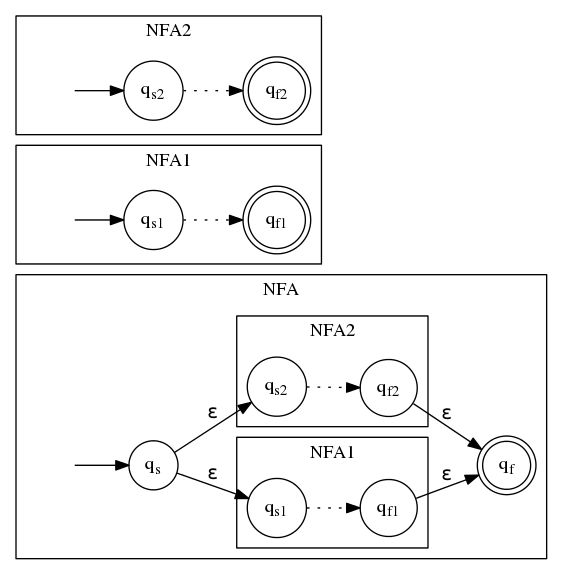
\includegraphics[width=0.5\textwidth]{assets/nfa_unie.png}      
      \caption{De unie van twee NFA's}
      \label{fig:nfa_unie}
    \end{figure}
    Formeel beschrijven we $n$ als volgt.
    \begin{itemize}
    \item $Q = Q_{1} \cup Q_{2} \cup \{ q_{s}, q_{f} \}$ waarbij $q_{s}$ en $q_{f}$ nieuwe toestanden zijn.
    \item $F = {q_{f}}$
    \item $\delta$ wordt aangepast als volgt:
      \begin{itemize}
      \item $\forall q \in Q_{i}\setminus\{q_{f_{i}}\},\ \forall x \in \Sigma_{\epsilon}:\ \delta(q,x) = \delta_{i}(q,x)$
      \item $\delta(q_{s},\epsilon) = \{q_{s1},q_{s2}\}$
      \item $\forall x \in \Sigma:\ \delta(q_{s},x) = \emptyset$
      \item $\delta(q_{f1},x) = \{q_{f}\}$ en $\delta(q_{f2},x) = \{q_{f}\}$
      \item $\forall x \in \Sigma:\ \delta(q_{f1},x) = \emptyset$, $\delta(q_{f2},x) = \emptyset$ en $\delta(q_{f},x) = \emptyset$ 
      \end{itemize}
    \end{itemize}
  \end{proof}
\end{st}

\begin{de}
  De \emph{concatenatie} $n_{1}n_{2}$ van twee NFA's $n_{1}$ en $n_{2}$ is de NFA $n$ die de concatenatie van de talen $L_{n_{1}}$ en $L_{n_{2}}$ aanvaardt.
\end{de}

\begin{st}
  \emph{Construtie van de concatenatie van twee NFA's}\\
  Het is steeds mogelijk om de concatenatie van twee NFA's te construeren.

  \begin{proof}
    Zij $n_{1} = (Q_{1},\Sigma,\delta_{1},q_{s1},\{q_{f1}\})$ en $n_{2} = (Q_{2},\Sigma,\delta_{2},q_{s2},\{q_{f2}\})$ twee willekeurige NFA's. We construeren nu de unie $n = n_{1}n_{2} = (O,\Sigma,\delta,q,\{q_{f}\})$ van deze NFA's.
    De informele constructie ziet u in figuur \ref{fig:nfa_concat}.
    \begin{figure}[H]
      \centering
      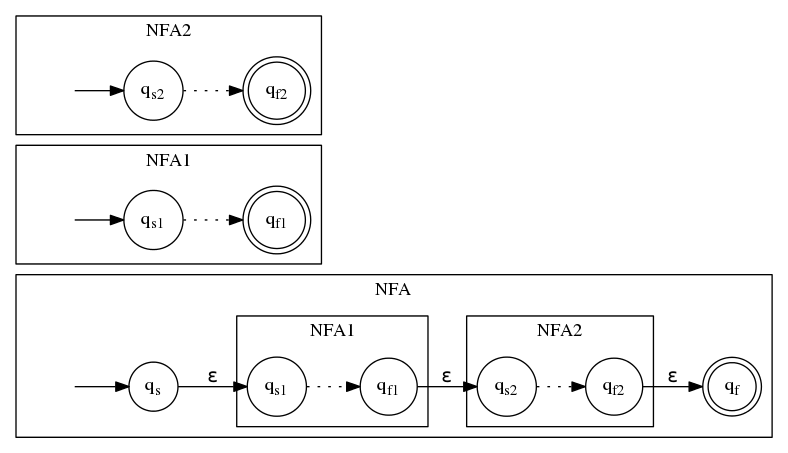
\includegraphics[width=0.7\textwidth]{assets/nfa_concat.png}      
      \caption{De concatenatie van twee NFA's}
      \label{fig:nfa_concat}
    \end{figure}
    Formeel beschrijven we $n$ als volgt.
    \begin{itemize}
    \item $Q = Q_{1} \cup Q_{2} \cup \{ q_{s}, q_{f} \}$ waarbij $q_{s}$ en $q_{f}$ nieuwe toestanden zijn.
    \item $F = {q_{f}}$
    \item $\delta$ wordt aangepast als volgt:
      \begin{itemize}
      \item $\forall q \in Q_{i}\setminus\{q_{f_{i}}\},\ \forall x \in \Sigma_{\epsilon}:\ \delta(q,x) = \delta_{i}(q,x)$
      \item $\delta(q_{s},\epsilon) = \{q_{s1}\}$
      \item $\forall x \in \Sigma:\ \delta(q_{s},x) = \emptyset$
      \item $\delta(q_{f1},\epsilon) = \{q_{s2}\}$
      \item $\delta(q_{s2},\epsilon) = \{q_{f}\}$
      \item $\forall x \in \Sigma:\ \delta(q_{f1},x) = \emptyset$, $\delta(q_{f2},x) = \emptyset$ en $\delta(q_{f},x) = \emptyset$ 
      \end{itemize}
    \end{itemize}
  \end{proof}
\end{st}

\begin{de}
  De \emph{Kleenester} van een NFA $n'$ is de NFA $n$ die de Kleenester van de taal $N_{n'}$ aanvaardt.
\end{de}

\begin{st}
  \emph{Construtie van de Kleenester van een NFA}\\
  Het is steeds mogelijk om de Kleenester van een NFA te construeren.

  \begin{proof}
    Zij $n' = (Q',\Sigma,\delta',q_{s},\{q_{f}'\})$ een willekeurige NFA. We construeren nu de Kleenester $n = (O,\Sigma,\delta,q,F)$ van deze NFA.
    De informele constructie ziet u in figuur \ref{fig:nfa_kleene}.
    \begin{figure}[H]
      \centering
      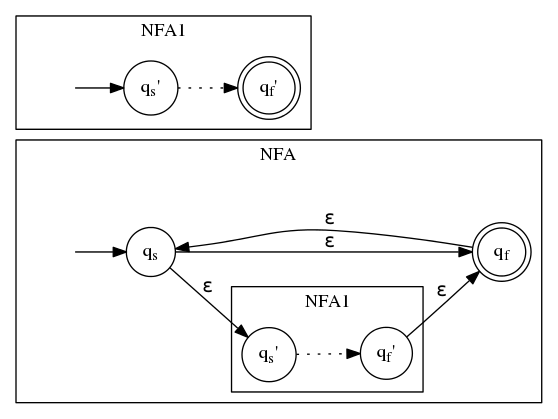
\includegraphics[width=0.5\textwidth]{assets/nfa_kleene.png}      
      \caption{De Kleenester van een NFA}
      \label{fig:nfa_kleene}
    \end{figure}
    Formeel beschrijven we $n$ als volgt.
    \begin{itemize}
    \item $Q = Q' \cup \{ q_{s}, q_{f} \}$ waarbij $q_{s}$ en $q_{f}$ nieuwe toestanden zijn.
    \item $F = {q_{f}'}$
    \item $\delta$ wordt aangepast als volgt:
      \begin{itemize}
      \item $\forall q \in Q'\setminus\{q_{f}'\},\ \forall x \in \Sigma_{\epsilon}:\ \delta(q,x) = \delta_{i}(q,x)$
      \item $\delta(q_{s},\epsilon) = \{q_{s}'\}$
      \item $\forall x \in \Sigma:\ \delta(q_{s},x) = \emptyset$
      \item $\delta(q_{f}',\epsilon) = \{q_{f}\}$
      \item $\delta(q_{f},\epsilon) = \{q_{s}\}$
      \item $\delta(q_{s},\epsilon) = \{q_{f}\}$
      \item $\forall x \in \Sigma:\ \delta(q_{f}',x) = \emptyset$ en $delta(q_{f},x) = \emptyset$
      \end{itemize}
    \end{itemize}
  \end{proof}
\end{st}

\end{document}
